\chapter{System Design}

\section{Business case}

ChatX is a chatting system which will allow users to communicate with each other from where ever they are and without fear of the messages being read by unwanted users, as long as they use a platform that supports the application and have a Internet connection.

\subsection{FURPS}
FURPS is a architectural checklist. It helps describe what areas needs to be focused on, and an overall view of what ChatX's purpose is.

\subsubsection{Functionality}
Functionality deals with requirements the customer has set for the project. To help the customer determine the requirements, a question to ask is: What problem is the system going to solve? And with ChatX, users that are in need of communication with other users from a long distance on a secure connection, making sure that messages are private, and only seen by the intended users.

\subsubsection{Usability}
Usability describes how accessible ChatX is for the users. Is it easy to use? Is the GUI design intuitive? A way to check if the users like the aesthetics of the application, and more importantly, can figure out how to use it, would be to prepare usability tests and alpha/beta tests as they can give crucial feedback on how user friendly the system is.

\subsubsection{Reliability} 
Reliability describes how reliable the system should be: How much downtime can it handle? Are failures predictable? How is the system going to recover in case of failure? 

Due to ChatX's architecture it is possible to setup several servers at once and if one fails, then the other servers can be used instead. In the worst case scenario - i.e. all servers shut down - then it would not take too long to install the server software on a different machine and ChatX would continue working.

\subsubsection{Performance}Performance describes how fast an application must be, what the highest allowed response time is and how much memory is needed. 

ChatX is a chatting system, meaning that messages has to be sent and received as quickly as possible, however we can only assure a fast reliable service at the server end.
%however it is impossible to assure that since it is unknown how good internet connections the users have.

\subsubsection{Supportability}
Supportability, the last of the FURPS principles, describes how maintainable an application is after deployment. It also describes how easy it is to install and configure. 

For ChatX, two installations are required: the server, and the client. The machine running the client also has to install java, and the machine(s) running the server and service has to have access to a supported message queue system.
 
 %ChatX has been developed with expansion in mind, as earlier mentioned in case of server side errors, another one can easily take its place. The same principle applies here, if for whatever a reason someone chooses to shut down the server, it would be easy to simple install the server software on a different machine.

\section{Architecture}
ChatX's architecture will be a client-server architecture. The client will call the server whenever a user requests to use the system and the server will keep track of how many users are online and where each message is supposed to be sent to.

\subsection{Domain Model}

\begin{figure}[H]
\centering
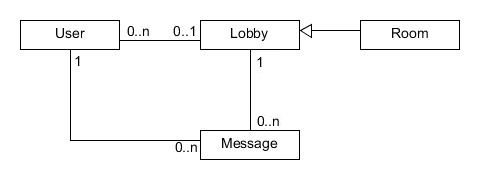
\includegraphics[width=0.7\linewidth]{img/DomainModelChatX}
\caption{Domain Model over ChatX}
\label{fig:DomainModelChatX}
\end{figure}

The domain model consists of four classes. The user class is where users are identified and if they are regular users or administrative users, a user can only be in one lobby at a time but a lobby can have multiple users. A user can also send zero to many messages. The message class is used for sending messages between users, a user can have zero to many messages, whilst a message can only belong to one user. The lobby is where all users start. From the lobby a user can create a room and choose which users are to be included in it, Or join a room. The room class inherits the functionality of the lobby class.

\clearpage
\subsection{Communicationdiagram}

\begin{figure}[h]
\centering
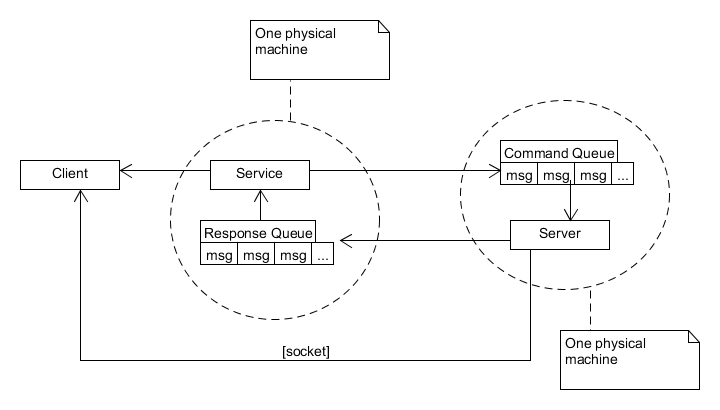
\includegraphics[width=0.7\linewidth]{img/CommunicationDiag}
\caption[Communication-diagram]{Communication-diagram}
\label{fig:Communicationdiagram}
\end{figure}

As seen in the diagram above, figure \ref{fig:Communicationdiagram}, the client asks for information at the service. The service then communicates with the queue system, in this case RabbitMQ, that then communicates with the server. The server always listens to queues that is in RabbitMQ, and as soon as a new message is in the command queue, which is the implemented way of saying messages that has not been dealt with yet, then it sends the messages out to those people who is in the room using the socket connection which is open constantly from the server to each of the clients.

\section{Cryptography}

To make the communication secure the clients implements an RSA encryption to encrypt all messages sent. RSA is a Public- Private key (asymmetric) encryption algorithm. RSA encryption is a standard for encrypting and is practically impossible to decode due to prime factorization. The general idea is that it is easy to find the product of two large primes, but it is hard to factor a large product and find the primes.

RSA was originally made by Ronald Linn Rivest along with Adi Shamir and Len Adlemanand published in their paper A Method for Obtaining Digital Signatures and Public-Key Cryptosystems\cite{RSA}.

To be able to apply RSA encryption, 6 variables are needed; $d$, $e$, $n$, $p$, $q$ and $\varphi$(phi). $d$, $p$, $q$ and $\varphi$(phi) should be kept secret at all time to keep this encryption secure. Let $p$ and $q$ be a prime number, lets for simplicity say $p=7$ and $q=13$. In practice these 2 numbers would be larger depending on the numbers of bits used for encryption. $n$ is defined as in equation \ref{RSA:n}.

\begin{equation}
n = p \times q
\label{RSA:n}
\end{equation}

In this case $n=91$. Additional $n$ have the bit-length dependent on security of the encryption. If the encryption should be 1024 bit, when $n$ would be a 1024 bit number. $\varphi$ or $\varphi(n)$ is found by using equation \ref{RSA:phi}.

\begin{equation}
\varphi = (p-1)(q-1)
\label{RSA:phi}
\end{equation}

For this example $\varphi = 72$ and it is now possible to find $e$ which is the public exponent. $e$ is a random prime and have two requirements which must be met; $e$ must be a relative prime of $\varphi$, ie. $e$ and $\varphi$ have no common factors and $e$ must be an integer such that $1 < e < \varphi$ and gcd$(e,\varphi)=1$. For this example let $e=7$. The public key is now available as $n$ and $e$ is known and can be given out.

Lastly we calculate $d$ which is the private exponent using extended euclidean algorithm. Equation \ref{RSA:d} is used for finding $d$.

%https://www.youtube.com/watch?v=moqmFy39Itc
\begin{equation}
d = e^{-1} \textrm{ mod } \varphi
\label{RSA:d}
\end{equation}

From equation \ref{RSA:d} $d=31$ and it is possible to further check if this is correct by using equation \ref{RSA:check} which in this case it is, and the private key is now defined by $n$ and $d$.

\begin{equation}
e \times d \textrm{ mod } n = 1
\label{RSA:check}
\end{equation}

Now where both the public and private keys are assigned, they can be used to encrypt and decrypt messages. If the message "Hi" were to be decrypted it would first need to be translated into a number, eg. as 8 and 9. It is now possible to encrypt both letter individually by using equation \ref{RSA:Encrypt} which gives the output cipher text $C$, and as well as decrypt it again with equation \ref{RSA:Decrypt}.

\begin{equation}
C=M^e \textrm{ mod } n \quad \textrm{Where M $<$ n}
\label{RSA:Encrypt}
\end{equation}

\begin{equation}
M=C^d \textrm{ mod } n
\label{RSA:Decrypt}
\end{equation}

In the computer world when encrypting data, a padding is often used. Padding is often used to fill out byte blocks. For instance, if the message "Hi!" would had the byte block [48 69 21]. This block size is only of 3 bytes, but the encryption algorithm might read a block of 8 at a time which would mean the block needs 5 more bytes. There is multiple ways of padding a message, such as zero-padding [48 69 21 00 00 00 00 00], padding with the same value as the number of bytes [48 69 21 05 05 05 05 05]\cite{PADDING}. When the padding is done a block can be sent to the encryption algorithm to produce the cipher text.